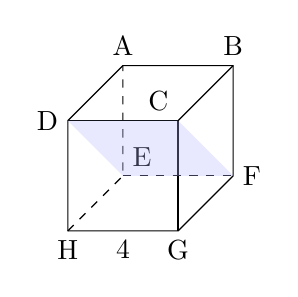
\begin{tikzpicture}
\draw(0,0)node[anchor=north]{H}--(0.7,0)node[anchor=north]{$4$}--(1.4,0)node[anchor=north]{G}--(2.1,0.7)node[anchor=west]{F}--(2.1,2.1)node[anchor=south]{B}--(0.7,2.1)node[anchor=south]{A}--(0,1.4)node[anchor=east]{D}--cycle;
\draw(0,1.4)--(1.4,1.4)node[anchor=south east]{C}--(1.4,0);
\draw(1.4,1.4)--(2.1,2.1);
\draw(0.7,0.7)node[anchor=south west]{E};
\draw[dashed](0,0)--(0.7,0.7)--(0.7,2.1);
\draw[dashed](0.7,0.7)--(2.1,0.7);
\fill[opacity=0.3,blue!30!white](0,1.4)--(1.4,1.4)--(2.1,0.7)--(0.7,0.7)--cycle;
\end{tikzpicture}
Note: diagram is \textbf{NOT} to scale.

Cube ABCDEFGH is bisected by plane CDEF resulting in two triangular
prisms as shown above. What is the volume of prism ABCDEF?



\ifsat
	\begin{enumerate}[label=\Alph*)]
		\item $8$
		\item $16$
		\item $32$%
		\item $64$
	\end{enumerate}
\else
\fi

\ifacteven
	\begin{enumerate}[label=\textbf{\Alph*.},itemsep=\fill,align=left]
		\setcounter{enumii}{5}
		\item $8$
		\item $16$
		\item $32$%
		\addtocounter{enumii}{1}
		\item $64$
		\item $128$
	\end{enumerate}
\else
\fi

\ifactodd
	\begin{enumerate}[label=\textbf{\Alph*.},itemsep=\fill,align=left]
		\item $8$
		\item $16$
		\item $32$%
		\item $64$
		\item $128$
	\end{enumerate}
\else
\fi

\ifgridin
 $32$%
		
\else
\fi

